\documentclass[12pt]{article}
\usepackage{arxiv}
\usepackage[utf8]{inputenc}
\usepackage[T1]{fontenc}
\usepackage{lmodern}
\usepackage{geometry}
\usepackage{hyperref}
\usepackage{graphicx}
\usepackage{booktabs}
\usepackage{array}
\usepackage{longtable}
\usepackage{enumitem}
\usepackage{xcolor}
\usepackage{listings}
\usepackage{amsmath}
\geometry{margin=1in}
\hypersetup{colorlinks=true,linkcolor=blue,urlcolor=blue,citecolor=blue}
\lstset{basicstyle=\ttfamily\small,breaklines=true,frame=single,columns=fullflexible}

\title{Laporan Proyek Mata Kuliah Rekayasa Perangkat Lunak \\\Large\textbf{MATCS: Multi-Agent Traffic Control System}}

\author{%
Samuel Tanaka Sibarani (2206059710)\\
Alfonsus Tanara G (2306267126)\\
Ade Zaskia Azzahra (2406344353)\\
Prof. Dr. Ir. Riri Fitri Sari, M.M., M.Sc. (RFS)\\
\textit{Departemen Teknik Elektro, Fakultas Teknik, Universitas Indonesia}\\
2026
}
\date{}

\begin{document}
\begin{center}

\includegraphics[width=0.25\textwidth]{logo_ui.png}
\end{center}
\vspace{0.5em}
\maketitle

\begin{abstract}
Laporan ini mendokumentasikan MATCS (Multi-Agent Traffic Control System), sebuah proyek rekayasa perangkat lunak untuk mengembangkan sistem pengendalian lalu lintas berbasis simulasi. Sistem dibatasi pada satu persimpangan dengan empat pendekat, kedatangan kendaraan yang dapat direproduksi, pengendali fixed-time, pengendali queue-aware heuristic, validator keselamatan deterministik, aktuator simulasi, serta metrik evaluasi. Implementasi awal menggunakan Python standard library tanpa koneksi ke perangkat lampu lalu lintas, jaringan publik, atau sistem otoritas. Laporan ini memperbarui rancangan awal dengan bukti implementasi, 13 pengujian otomatis, dan 80 eksperimen terkontrol. Hasil awal menunjukkan bahwa heuristik queue-aware menjanjikan pada permintaan yang tidak seimbang, tetapi belum dapat diklaim lebih baik secara universal. Bab tambahan membahas project plan, UML, rancangan MoU, estimasi COCOMO, dan Function Point Analysis.
\end{abstract}

\newpage
\section*{Abstract (English)}
This report documents MATCS (Multi-Agent Traffic Control System), a software-engineering project for simulation-based traffic control. The current scope is one four-approach intersection with reproducible vehicle arrivals, fixed-time and queue-aware heuristic controllers, a deterministic safety validator, a simulated actuator, and evaluation metrics. The implementation uses only the Python standard library and does not connect to traffic-light hardware, public networks, or authority systems. This report updates the initial design with implementation evidence, 13 automated tests, and 80 controlled experiment runs. Initial results suggest that the queue-aware heuristic is promising under directional imbalance but cannot yet be claimed universally superior. Additional chapters cover the project plan, UML, a draft MoU, COCOMO estimation, and Function Point Analysis.

\newpage
\tableofcontents
\listoffigures
\listoftables

\section*{Daftar Singkatan dan Istilah}
\begin{itemize}[leftmargin=1.2em]
  \item MATCS: Multi-Agent Traffic Control System.
  \item UML: Unified Modeling Language.
  \item MoU: Memorandum of Understanding.
  \item COCOMO: Constructive Cost Model.
  \item FPA: Function Point Analysis.
  \item CLI: Command-Line Interface.
  \item Queue-aware: pengendali yang menggunakan panjang antrean dan waktu tunggu untuk memilih fase berikutnya.
  \item Shadow mode: mode rekomendasi tanpa mengambil alih sistem lapangan.
\end{itemize}

\newpage
\section{BAB 1. PENDAHULUAN}
\subsection{Latar Belakang}
Kemacetan perkotaan berubah menurut waktu, pola perjalanan, aktivitas publik, cuaca, dan insiden. Pengaturan lampu lalu lintas yang sepenuhnya tetap dapat memberikan waktu hijau yang tidak sebanding dengan permintaan aktual. Akibatnya, suatu pendekat dapat membentuk antrean sementara pendekat lain belum menggunakan kapasitasnya.

Masalah ini menjadi lebih kompleks ketika beberapa persimpangan berada dalam satu koridor. Keputusan yang mengurangi antrean pada satu persimpangan dapat memindahkan beban ke persimpangan berikutnya. Karena itu, MATCS dirancang sebagai studi rekayasa perangkat lunak yang memisahkan observasi, pembentukan state, proposal pengendali, validasi keselamatan, aktuasi, dan evaluasi.

\subsection{Identifikasi Masalah}
Masalah utama proyek adalah bagaimana membangun prototipe pengendalian lalu lintas yang dapat diuji secara aman, murah, dan dapat direproduksi. Sistem harus mampu membandingkan kebijakan pengendali pada kondisi permintaan yang sama, mencatat metrik secara konsisten, dan mencegah proposal fase yang melanggar urutan keselamatan.

\subsection{Rumusan Masalah}
\begin{enumerate}
  \item Bagaimana membangun simulator satu persimpangan yang deterministik dan mudah ditinjau oleh tiga mahasiswa?
  \item Bagaimana membandingkan fixed-time controller dan queue-aware heuristic secara adil?
  \item Bagaimana menerapkan batas keselamatan deterministik sebelum aktuasi simulasi?
  \item Bagaimana mendokumentasikan project plan, UML, MoU, COCOMO, dan FPA secara konsisten dengan implementasi?
\end{enumerate}

\subsection{Tujuan}
Tujuan utama adalah mengembangkan dan mengevaluasi vertical slice MATCS untuk satu persimpangan. Tujuan teknisnya adalah menyediakan simulator lokal, controller baseline, heuristic controller, safety validator, metrics collector, automated tests, dan batch experiment runner.

\subsection{Ruang Lingkup dan Batasan}
Ruang lingkup saat ini meliputi satu persimpangan empat pendekat, empat demand profile, dua controller, synthetic arrivals, simulasi fase, metrik antrean dan delay, serta output CSV/JSON. Sistem tidak mengendalikan lampu lalu lintas nyata, tidak membaca kabinet sinyal, tidak melakukan koneksi authority gateway, dan tidak mengklaim keselamatan untuk deployment.

\subsection{Metodologi}
Pengembangan dilakukan secara iteratif: definisi kontrak, implementasi vertical slice, pengujian, eksperimen matched-seed, interpretasi hasil, dan revisi dokumentasi. Semua percobaan dapat diulang menggunakan seed, durasi, demand profile, dan controller yang tercatat.

\subsection{Sistematika Penulisan}
Bab 1 menjelaskan konteks. Bab 2 membahas dasar teori dan teknologi. Bab 3 berisi project plan dan UML. Untuk sementara, materi analisis kebutuhan, arsitektur, MoU, estimasi, implementasi, pengujian, dan hasil ditempatkan sebagai sub-bab pada Bab 4 sampai ada instruksi struktur lebih lanjut dari dosen. Bab 5 berisi kesimpulan sementara.

\section{BAB 2. TINJAUAN PUSTAKA}
\subsection{Adaptive Traffic Control}
Adaptive traffic control menggunakan observasi permintaan untuk menyesuaikan keputusan fase. Dalam proyek ini, adaptivitas pertama diwujudkan melalui heuristic queue-aware, bukan model machine learning.

\subsection{Multi-Agent Software Architecture}
Istilah multi-agent digunakan untuk memisahkan tanggung jawab: observation/state adapter, intersection controller, safety validator, simulated actuator, dan evaluation module. Pada satu persimpangan seluruh komponen berjalan sebagai modul dalam satu proses lokal. Deployment terpisah dan koordinasi antar-persimpangan ditunda.

\subsection{Deterministic Safety Boundary}
Controller hanya menghasilkan proposal abstrak berupa fase saat ini atau fase berikutnya. SafetyValidator menolak timestamp yang stale dan transisi yang melewati fase. Aturan ini tetap berlaku jika controller pada masa depan diganti optimizer atau learned policy.

\subsection{Estimasi Perangkat Lunak}
COCOMO dan FPA digunakan sebagai alat perencanaan, bukan sebagai bukti biaya aktual. Nilainya bergantung pada ukuran kode, kompleksitas, tingkat pengalaman tim, dan batasan akademik. Oleh sebab itu, asumsi perhitungan disajikan secara eksplisit pada Bab 4.

\section{BAB 3. PROJECT PLAN DAN UML}
\subsection{Pendekatan Manajemen Proyek}
Tim menggunakan proses iteratif ringan dengan Trello sebagai sumber kebenaran project management dan GitHub sebagai sumber kebenaran kode serta dokumentasi. Setiap pekerjaan memiliki tujuan, owner, acceptance evidence, review, dan catatan risiko.

\subsection{Struktur Tim dan Tanggung Jawab}
\begin{longtable}{p{0.25\textwidth} p{0.65\textwidth}}
\toprule
\textbf{Anggota} & \textbf{Tanggung jawab utama}\\
\midrule
Samuel Tanaka Sibarani & Koordinasi, integrasi report, simulator, eksperimen, dan administrasi project board.\\
Alfonsus Tanara G & Riset controller, safety boundary, desain eksperimen, dan review teknis.\\
Ade Zaskia Azzahra & Dokumentasi, UML, project evidence, dan review kebutuhan/presentasi.\\
\bottomrule
\end{longtable}

\subsection{Fase dan Milestone}
\begin{longtable}{p{0.18\textwidth} p{0.70\textwidth}}
\toprule
\textbf{Fase} & \textbf{Deliverable dan acceptance evidence}\\
\midrule
Fase 0: Scope & Batas simulation-only, non-goals, risk register, dan repository setup.\\
Fase 1: Vertical slice & Models, fixed-time controller, validator, simulator, metrics, CLI.\\
Fase 2: Evidence & Queue-aware controller, demand profiles, 13 tests, CSV/JSON batch results.\\
Fase 3: Review & UML, report, interpretation, code review, dan demonstrasi lokal.\\
Fase 4: Future research & Statistical evaluation, calibrated digital twin, lalu possible shadow mode dengan persetujuan terpisah.\\
\bottomrule
\end{longtable}

\subsection{Jadwal dan Definition of Done}
Pekerjaan dinyatakan selesai apabila implementasi berjalan, test atau evidence tersedia, anggota lain dapat meninjau hasilnya, dokumentasi diperbarui, dan risiko tindak lanjut dicatat. Fase berikutnya tidak boleh menghapus fixed-time baseline atau safety validator.

\newpage
\subsection{UML 1: Use-Case Diagram}
Aktor utama adalah student developer dan lecturer/reviewer. Authority/site stakeholder hanya berinteraksi pada batas future observation approval, bukan sebagai asumsi hak aktuasi.
\begin{figure}[htbp]
\centering
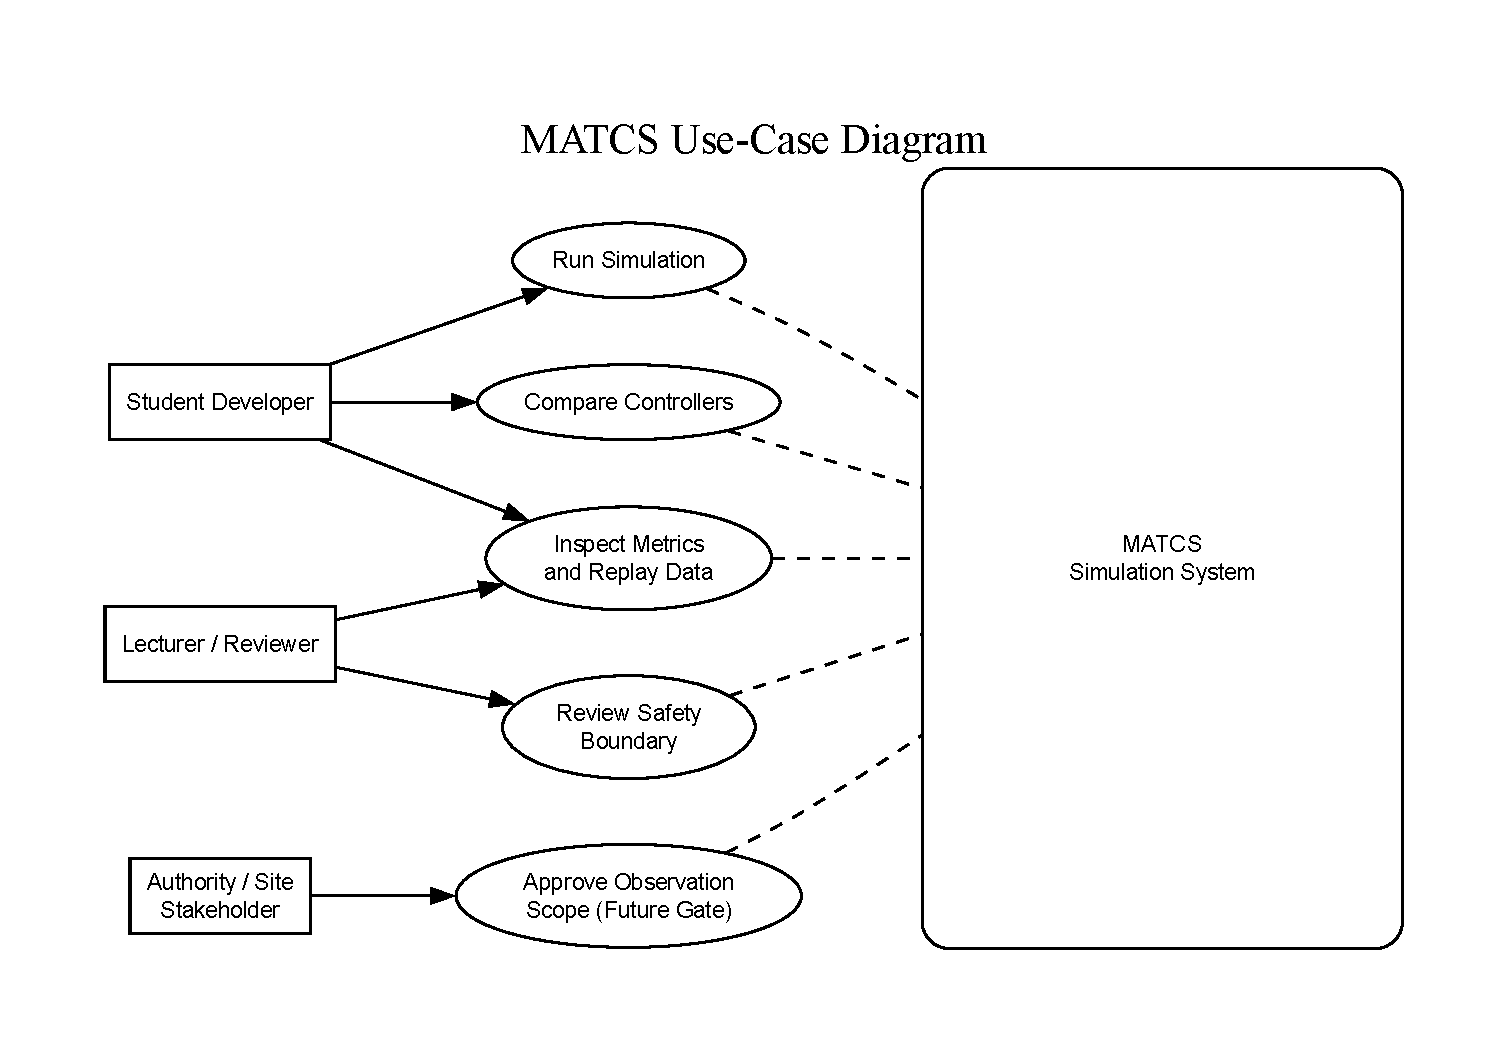
\includegraphics[width=0.95\textwidth]{figures/use-case.pdf}
\caption{Use-case diagram MATCS.}
\label{fig:use-case}
\end{figure}

\newpage
\subsection{UML 2: Class Diagram}
Kelas utama adalah ScenarioConfig, DemandProfile, TimingPlan, SimulationState, SignalState, FixedTimeController, QueueAwareController, SafetyValidator, SimulatedActuator, TrafficSimulator, MetricsCollector, dan RunMetrics.
\begin{figure}[htbp]
\centering
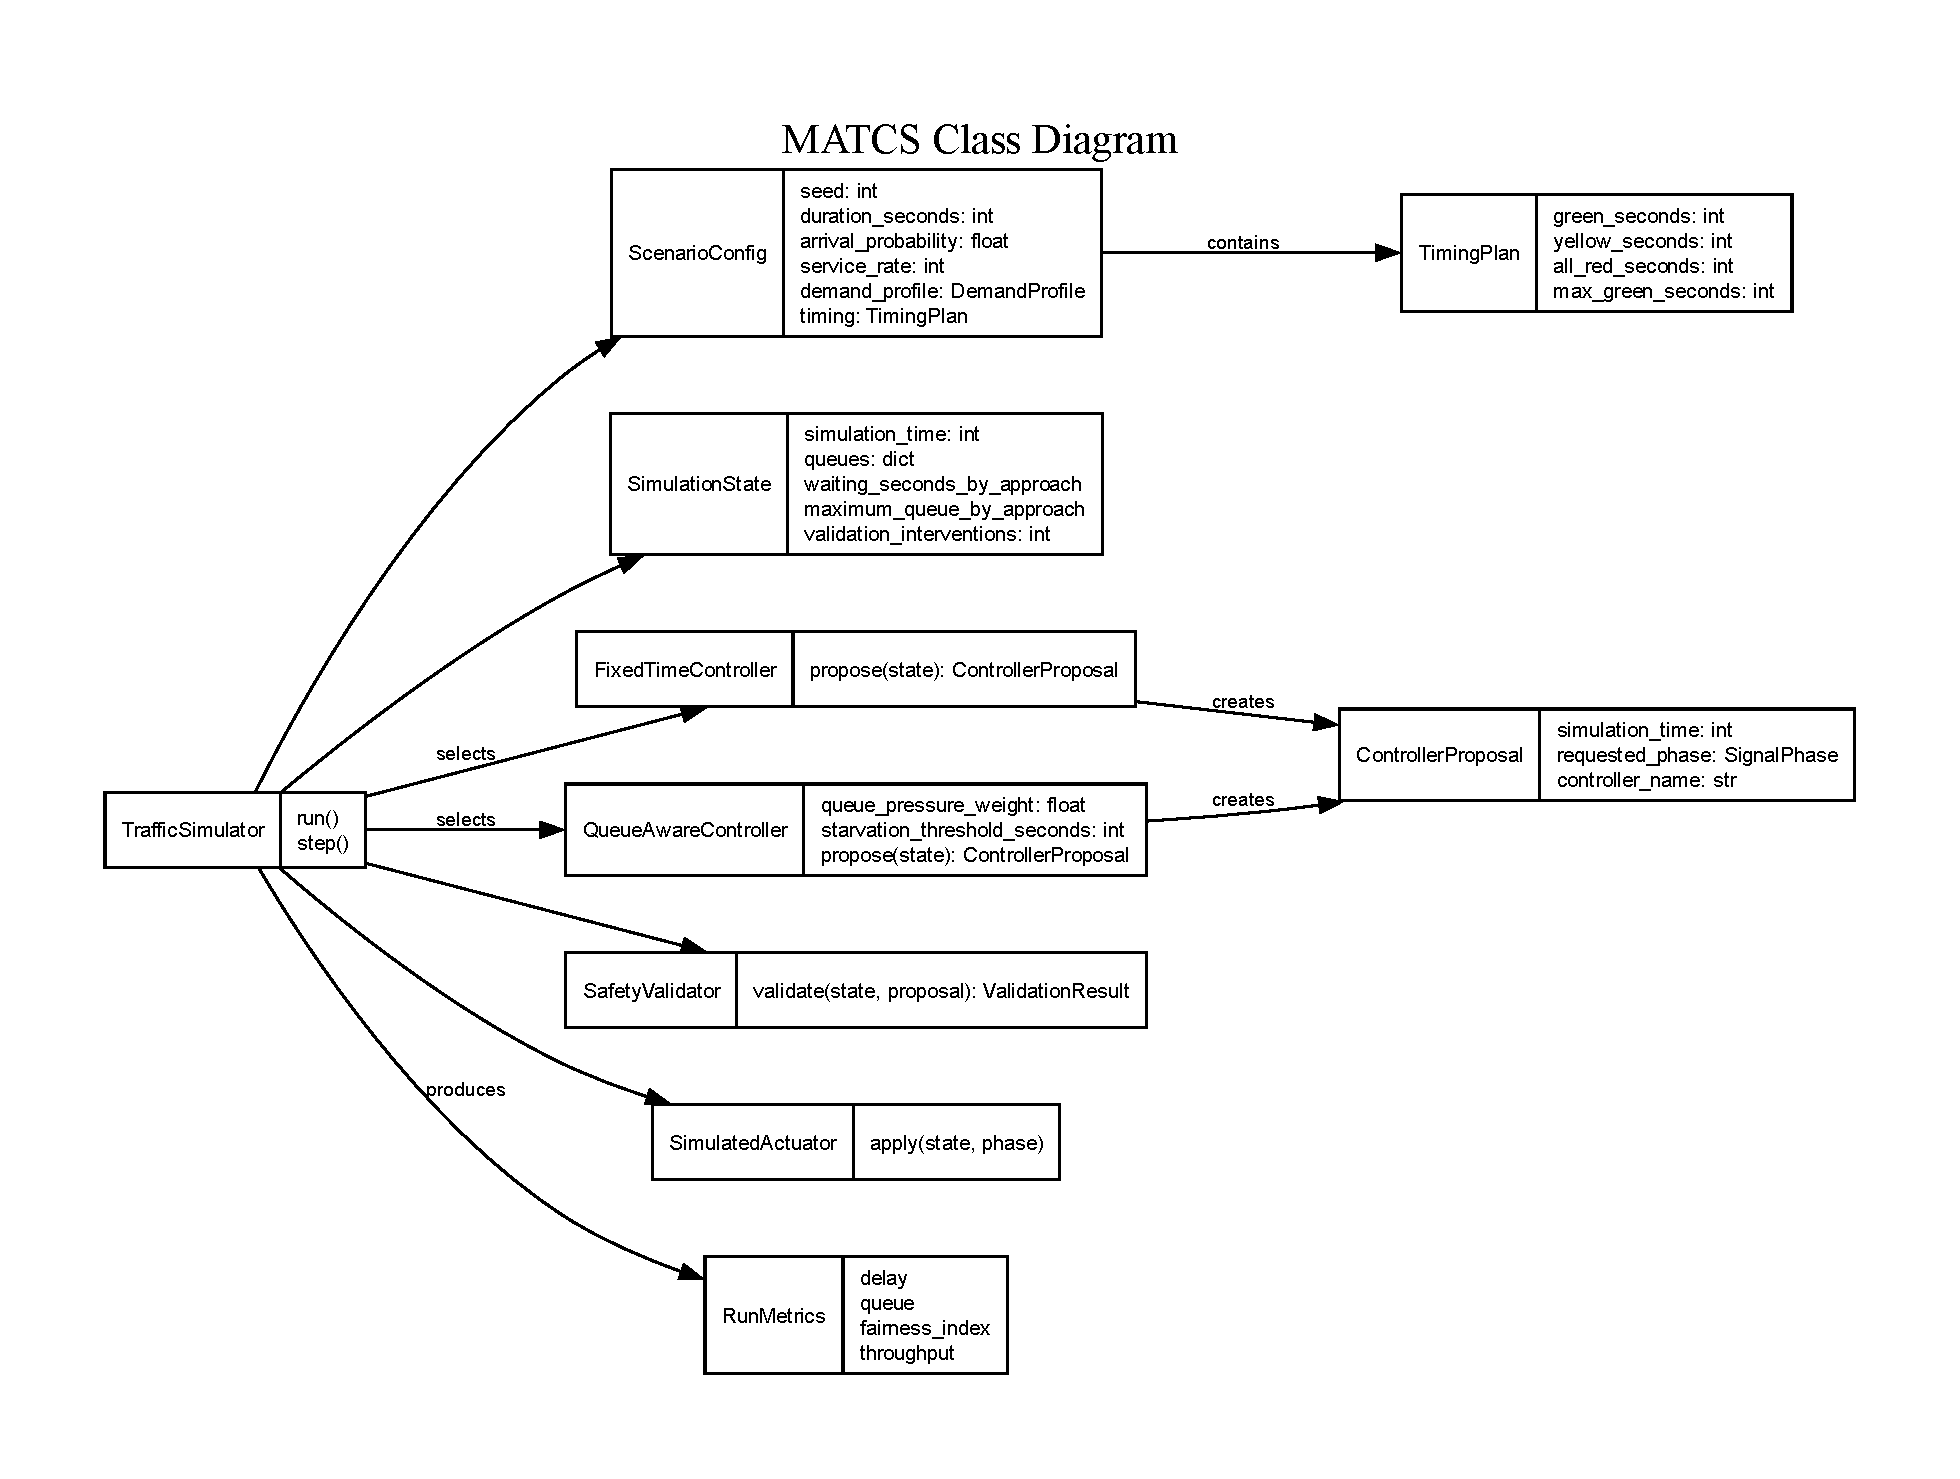
\includegraphics[width=\textwidth]{figures/class.pdf}
\caption{Class diagram MATCS.}
\label{fig:class}
\end{figure}

\newpage
\subsection{UML 3: Sequence Diagram}
Urutan satu tick adalah generate arrivals; controller propose; validator validate; actuator apply jika accepted; move vehicles; update waiting/delay; metrics observe; dan advance simulation time.
\begin{figure}[htbp]
\centering
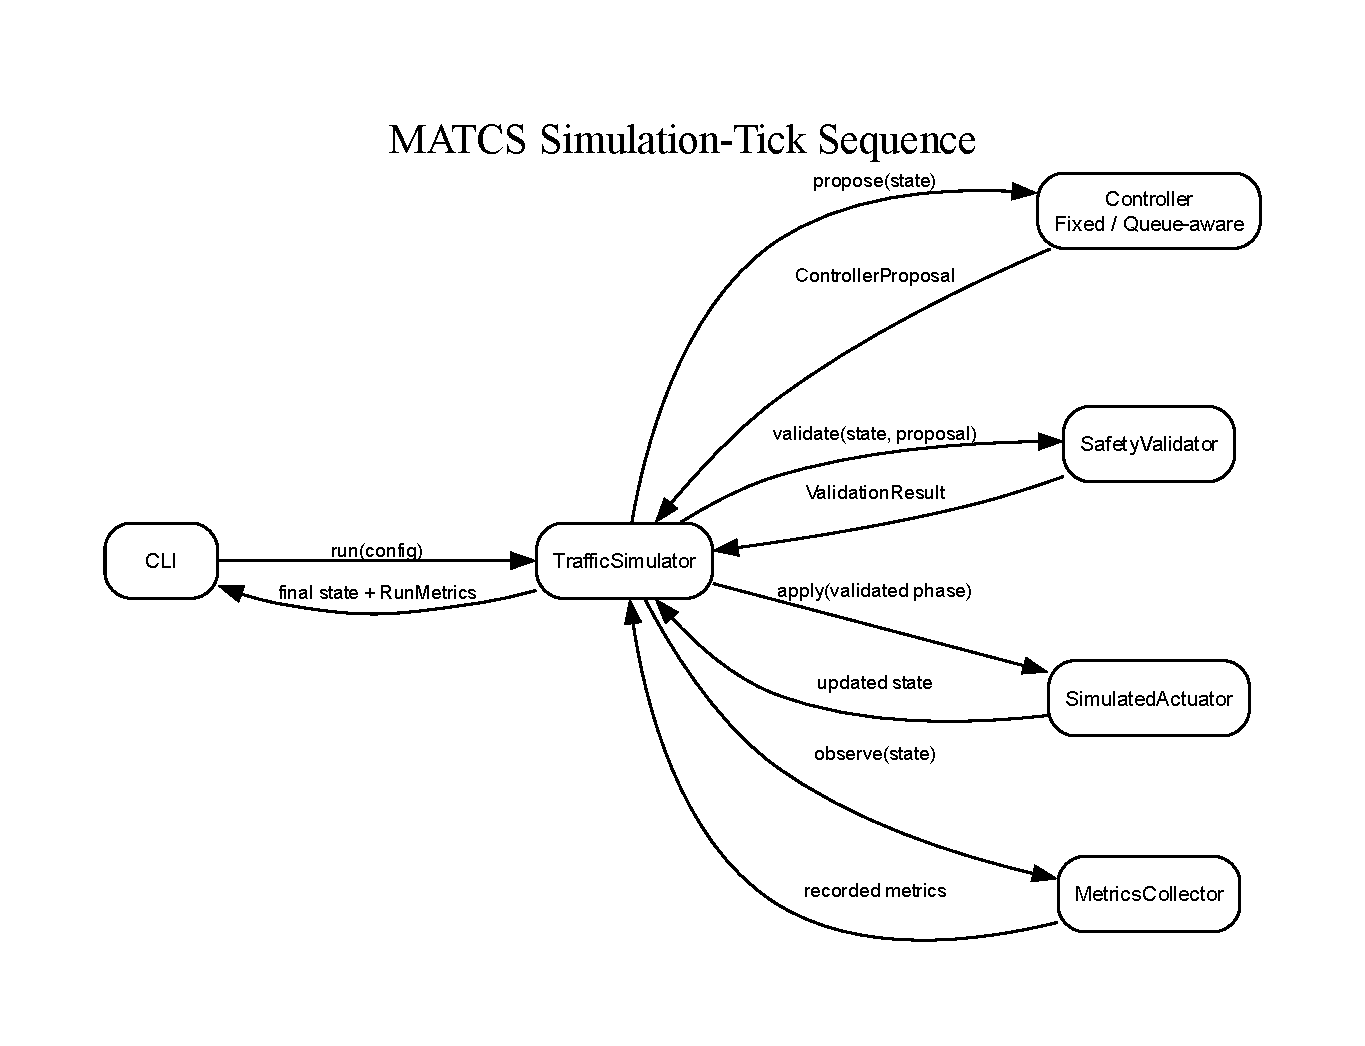
\includegraphics[width=\textwidth]{figures/sequence.pdf}
\caption{Sequence diagram satu simulation tick MATCS.}
\label{fig:sequence}
\end{figure}

\newpage
\subsection{UML 4: Activity Diagram}
Aktivitas dimulai dengan konfigurasi seed, durasi, demand profile, dan controller. Sistem melakukan loop tick sampai durasi selesai. Jalur accepted menuju simulated actuator, sedangkan jalur rejected mempertahankan fase aman dan mencatat intervention.
\begin{figure}[htbp]
\centering
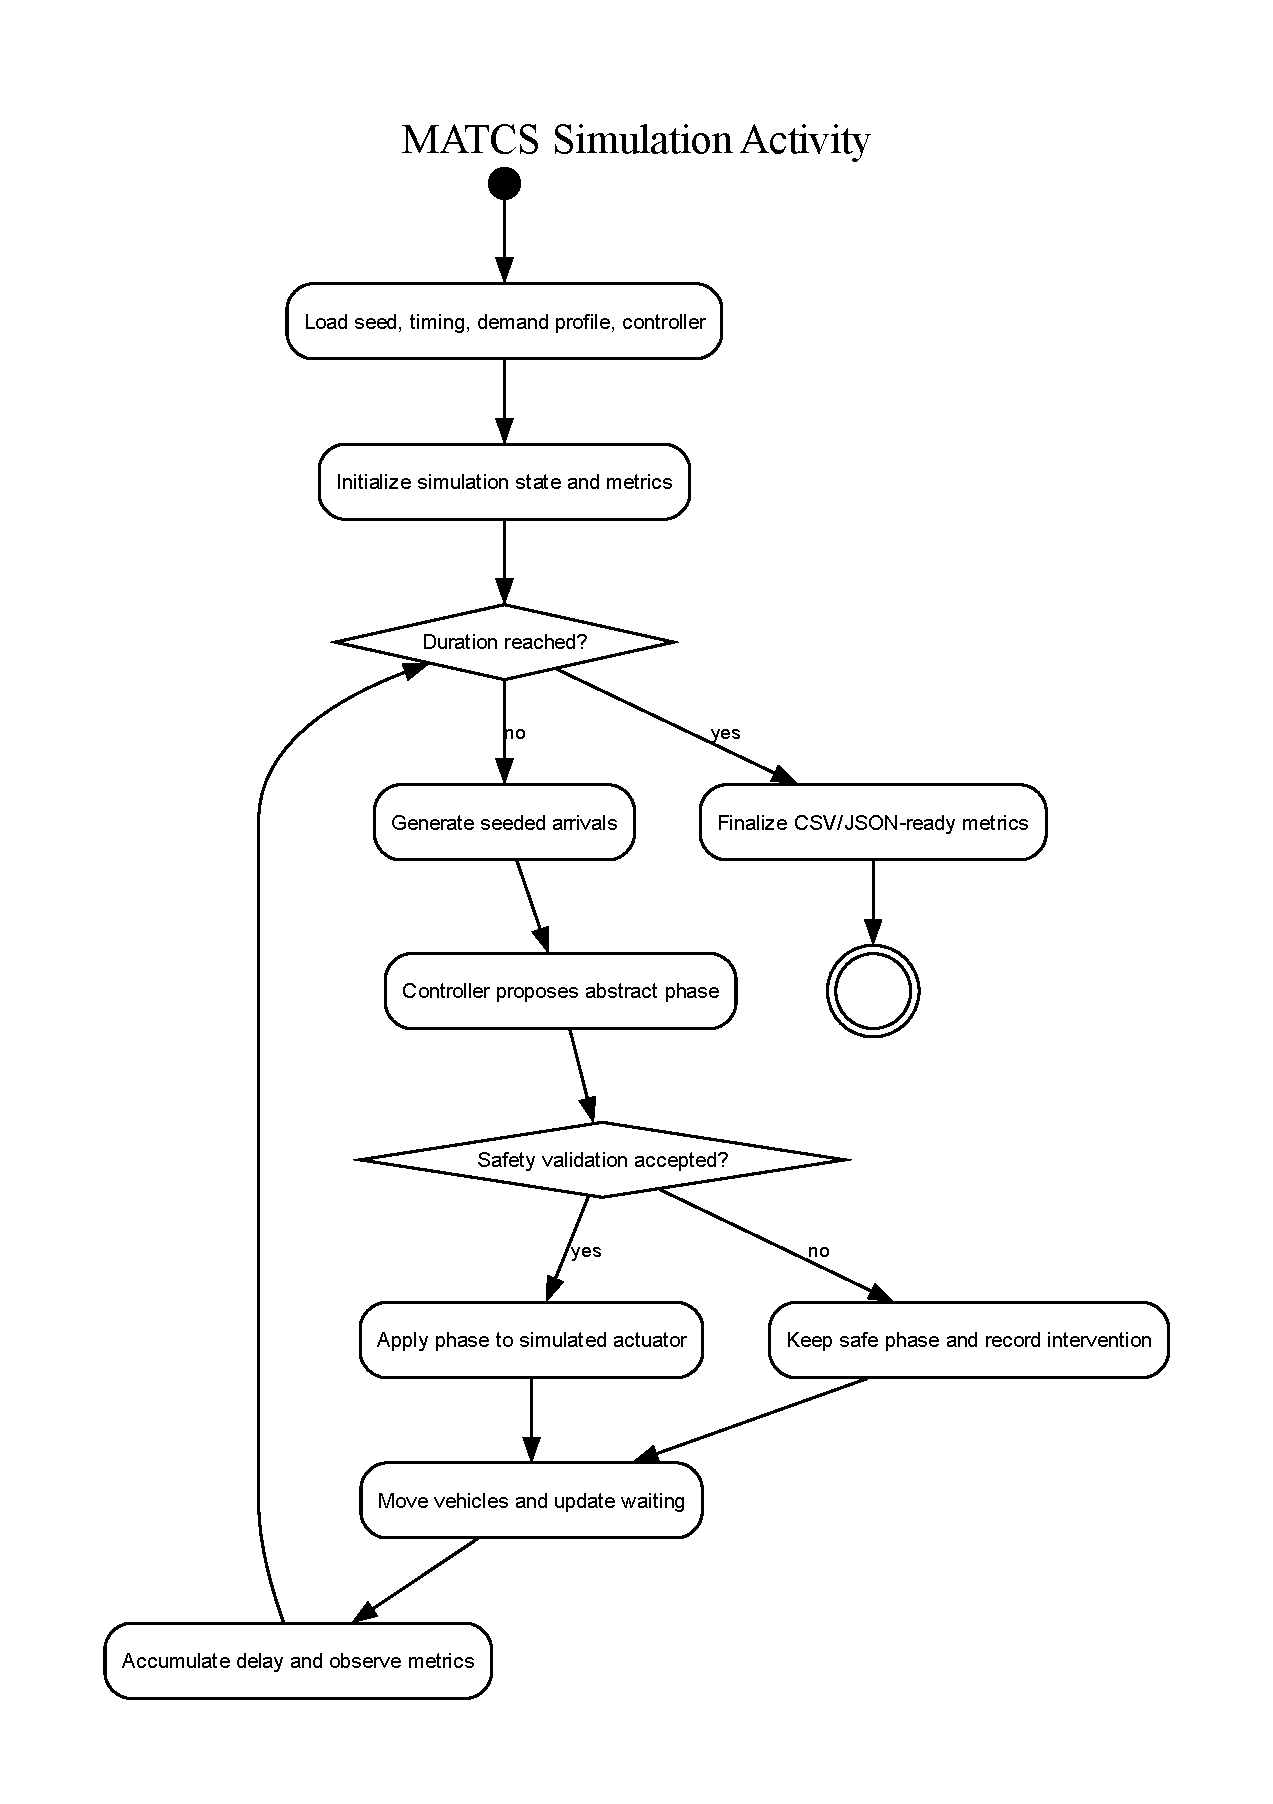
\includegraphics[width=0.75\textwidth]{figures/activity.pdf}
\caption{Activity diagram simulasi MATCS.}
\label{fig:activity}
\end{figure}

\newpage
\subsection{UML 5: State-Machine Diagram}
Urutan fase adalah North/South Green, North/South Yellow, All-Red to East/West, East/West Green, East/West Yellow, dan All-Red to North/South. Controller tidak dapat melompati yellow atau all-red.
\begin{figure}[htbp]
\centering
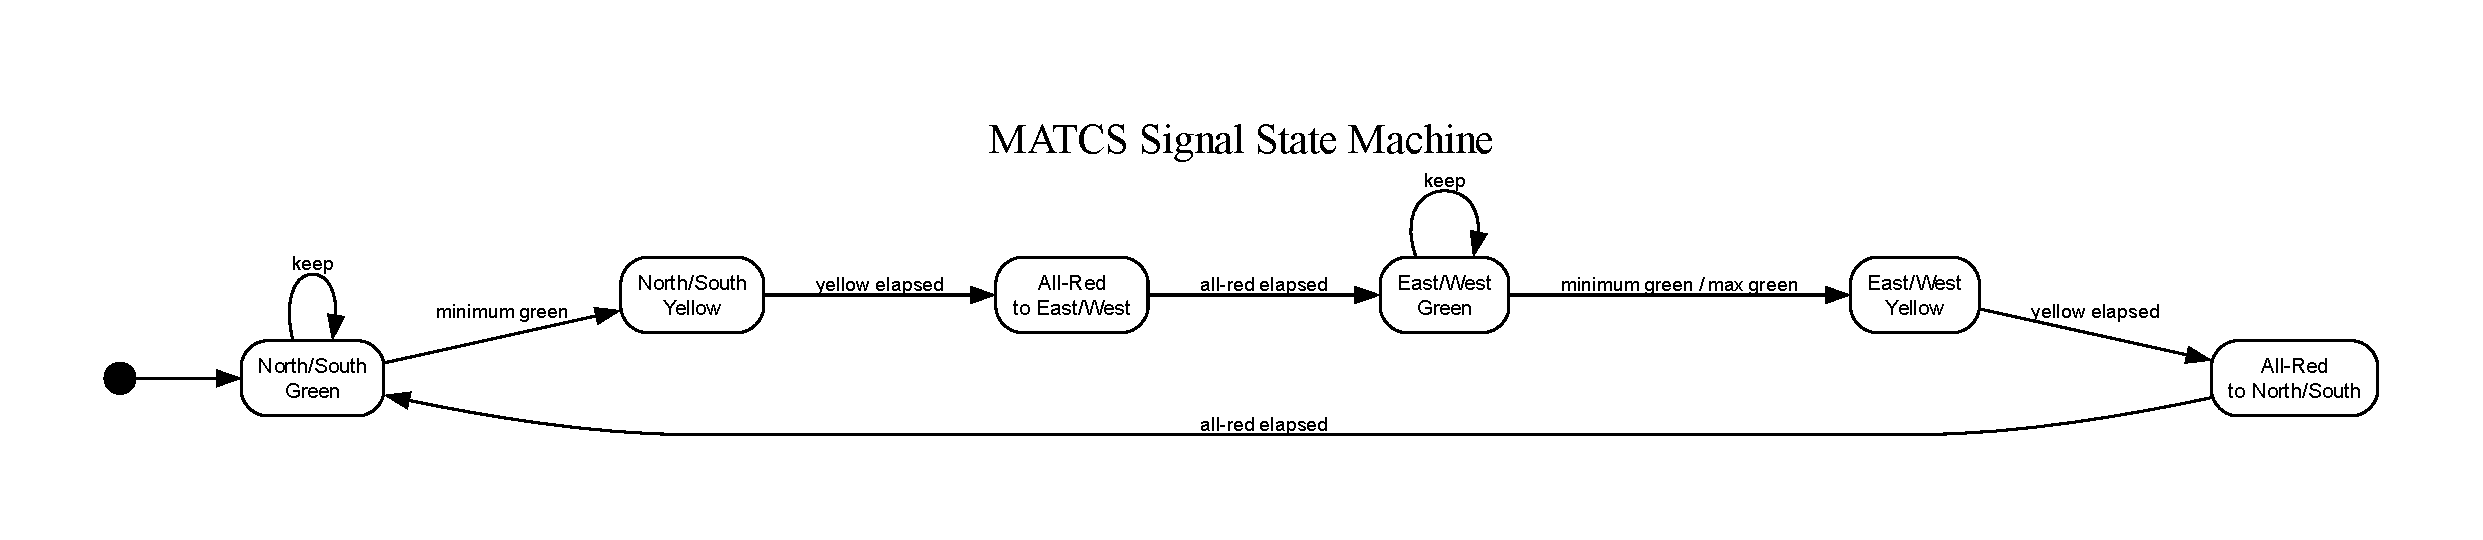
\includegraphics[width=\textwidth]{figures/state-machine.pdf}
\caption{State-machine diagram fase sinyal MATCS.}
\label{fig:state-machine}
\end{figure}

\subsection{UML Tambahan: Component dan Deployment}
Komponen tambahan adalah demand generator, observation adapter, state, controller strategy, safety validator, simulated actuator, metrics collector, CLI, dan future authority-approved observation adapter. Deployment saat ini hanya satu laptop dengan satu proses Python dan test runner lokal. Diagram editable lengkap tersedia pada `docs/11-uml-models.md` di repository.

\section{BAB 4. ANALISIS, PERENCANAAN, IMPLEMENTASI, DAN EVALUASI SEMENTARA}
\subsection{Memorandum of Understanding (MoU)}
Naskah MoU akademik telah disusun mengikuti format template dan tersedia sebagai dokumen Markdown terpisah pada \texttt{ClassGroup-Output/MoU-MATCS.md}. Dokumen tersebut mencakup identitas para pihak, tujuan dan ruang lingkup kolaborasi, jangka waktu, hak dan kewajiban, keselamatan dan data, kekayaan intelektual, keadaan kahar, perubahan, serta blok penutup dan tanda tangan.

Pihak pertama adalah Tim Proyek MATCS yang diwakili Samuel Tanaka Sibarani, dengan Alfonsus Tanara G dan Ade Zaskia Azzahra sebagai anggota tim. Pihak kedua adalah dosen pengampu/pembimbing, Prof. Dr. Ir. Riri Fitri Sari, M.M., M.Sc. (RFS). Nomor dokumen, kapasitas penandatangan, alamat/kontak, tempat, tanggal efektif, serta keterangan institusional yang belum tersedia ditandai sebagai isian untuk dikonfirmasi.

\textbf{Status MoU:} Naskah telah selesai disusun dan siap disampaikan kepada para pihak untuk ditinjau dan dilengkapi sebelum persetujuan/penandatanganan. Status complete pada laporan ini merujuk pada penyelesaian penyusunan dokumen, bukan persetujuan, tanda tangan, pengesahan, atau izin akses infrastruktur. MoU tidak memberi kewenangan observasi lapangan maupun aktuasi sinyal publik; setiap kegiatan di luar simulasi memerlukan persetujuan terpisah dan prosedur institusional/otoritas yang berlaku.

\subsection{COCOMO: Estimasi Awal}
Estimasi berikut menggunakan Basic COCOMO organic sebagai estimasi akademik awal. Ukuran asumsi adalah 2.5 KLOC equivalent untuk vertical slice Python, effort multiplier organic \(a=2.4\), \(b=1.05\), schedule \(c=2.5\), dan \(d=0.38\).

\[
E = 2.4(2.5)^{1.05} \approx 6.3\text{ person-months}
\]
\[
T = 2.5(E)^{0.38} \approx 4.9\text{ months}
\]

Angka ini bukan klaim durasi aktual tiga mahasiswa. Kode masih kecil, banyak aktivitas bersifat pembelajaran/dokumentasi, dan COCOMO tidak menangkap seluruh reuse standard library maupun kontribusi non-code. Dengan tiga anggota, angka effort kasar tersebut setara rata-rata sekitar 2.1 person-month per anggota sebelum memperhitungkan kalender kuliah.

\subsection{Function Point Analysis}
FPA berikut menggunakan pendekatan simplified IFPUG dengan bobot low complexity: External Input (EI)=3, External Output (EO)=4, External Inquiry (EQ)=3, Internal Logical File (ILF)=7, External Interface File (EIF)=5.

\begin{longtable}{p{0.48\textwidth} r r r}
\toprule
\textbf{Function} & \textbf{Count} & \textbf{Weight} & \textbf{Points}\\
\midrule
Scenario/controller configuration (EI) & 4 & 3 & 12\\
CLI run and experiment execution (EI) & 2 & 3 & 6\\
Metrics and comparison output (EO) & 5 & 4 & 20\\
State/metrics inspection (EQ) & 3 & 3 & 9\\
Simulation state and experiment records (ILF) & 3 & 7 & 21\\
Future approved observation input (EIF) & 1 & 5 & 5\\
\midrule
\textbf{Unadjusted Function Points} & & & \textbf{73}\\
\bottomrule
\end{longtable}

Dengan asumsi general system characteristics total 25 dari skala 0--5, value adjustment factor adalah \(0.65 + 0.01(25)=0.90\). Maka adjusted FP diperkirakan \(73\times0.90=65.7\), dibulatkan menjadi 66 FP. Nilai ini harus direvisi ketika dashboard, database, atau adapter lapangan benar-benar diimplementasikan.

\subsection{Analisis Kebutuhan dan Arsitektur}
\subsection{Kebutuhan Fungsional}
\begin{enumerate}
  \item Sistem dapat menjalankan simulasi dengan seed dan durasi tertentu.
  \item Sistem dapat memilih fixed-time atau queue-aware controller.
  \item Sistem dapat menghasilkan demand profile balanced, directional-heavy, dan stress.
  \item Sistem memvalidasi setiap proposal sebelum simulated actuation.
  \item Sistem menghasilkan arrivals, departures, queue, delay, stops, throughput, waiting, fairness, dan intervention metrics.
  \item Sistem dapat menghasilkan raw CSV dan summary JSON untuk matched experiments.
\end{enumerate}

\subsection{Kebutuhan Nonfungsional}
Reproducibility, local execution, no external dependency, safety-boundary separation, readable code, testability, dan traceability menjadi kebutuhan utama. Performance produksi dan real-time field reliability belum menjadi acceptance claim.

\subsection{Arsitektur}
Aliran utama adalah demand/observation menuju SimulationState, controller proposal, deterministic validator, simulated actuator, lalu metrics. Future field observation adapter hanya dapat ditambahkan melalui authority-approved gate dan tidak mengubah simulator menjadi pengendali publik secara otomatis.

\subsection{Implementasi Sistem}
\subsection{Lingkungan Pengembangan}
Implementasi menggunakan Python 3 dan standard library. Seluruh kode, test, scripts, dokumentasi, dan report source tersedia pada GitHub repository kelompok: \url{https://github.com/sammtan/MATCS}. Repository menggunakan struktur `src/mtacs` untuk package, `tests` untuk unittest, `scripts/run\_experiments.py` untuk batch experiment, dan `docs` untuk design records.

\subsection{Domain Models}
`Approach`, `SignalPhase`, `TimingPlan`, `ScenarioConfig`, `SimulationState`, `ControllerProposal`, `ValidationResult`, dan `RunMetrics` mendefinisikan kontrak domain. DemandProfile menyediakan probabilitas reproducible untuk balanced, directional-heavy, dan stress scenarios.

\subsection{Controllers and Safety}
FixedTimeController mengikuti urutan fase terkonfigurasi. QueueAwareController menggunakan queue pressure, waiting age, minimum green, maximum green, dan starvation threshold. Kedua controller hanya mengusulkan fase saat ini atau fase berikutnya. SafetyValidator memeriksa simulation time dan transisi fase.

\subsection{Metrics and Batch Runner}
MetricsCollector menghitung queue maximum, mean queue, accumulated delay, throughput, fairness index, per-approach waiting, per-approach maximum queue, dan validation interventions. Batch runner menjalankan kombinasi seed, durasi, profile, dan controller lalu menghasilkan `raw\_runs.csv` dan `summary.json`.

\subsection{Pengujian dan Validasi}
\subsection{Automated Tests}
Sebanyak 13 test berhasil dijalankan. Cakupannya meliputi transition, stale proposal, skipped phase, reproducibility, profile/duration matrix, matched controller inputs, stress scale, zero demand, fairness bounds, starvation protection, metrics keys, dan artifact schema.

\subsection{Acceptance Result}
Hasil final adalah `Ran 13 tests ... OK`. Seluruh test berjalan lokal tanpa dependency tambahan. Zero validation intervention pada batch runs menunjukkan proposal yang dihasilkan controller memenuhi kontrak transisi pada simulator; hasil ini bukan sertifikasi keselamatan dunia nyata.

\subsection{Hasil Eksperimen dan Pembahasan}
\subsection{Eksperimen}
Batch evidence terdiri dari 4 demand profile, 2 durasi (120 dan 600 detik), 5 seed, dan 2 controller, sehingga menghasilkan 80 runs. Perbandingan menggunakan profile, seed, duration, timing, service rate, dan topology yang sama.

\begin{longtable}{p{0.30\textwidth} r r r}
\toprule
\textbf{Metric} & \textbf{Balanced} & \textbf{North/South Heavy} & \textbf{East/West Heavy}\\
\midrule
Delay change & +1.84\% & -1.33\% & -5.77\%\\
Mean queue change & +1.83\% & -1.33\% & -5.77\%\\
Throughput change/min & -1.40 & 0.00 & +1.60\\
Fairness fixed $\rightarrow$ heuristic & 0.9782 $\rightarrow$ 0.9845 & 0.9747 $\rightarrow$ 0.9765 & 0.9153 $\rightarrow$ 0.9699\\
\bottomrule
\end{longtable}
\noindent\textit{Catatan:} Profil stress memiliki delay +2.00\%, mean queue +2.00\%, throughput -0.80 per menit, dan fairness 0.9931 $\rightarrow$ 0.9960; ditulis terpisah agar tabel tetap terbaca.

\subsection{Interpretasi}
Queue-aware paling menjanjikan ketika demand tidak seimbang, khususnya east/west-heavy. Namun balanced dan stress short-horizon mengalami regresi kecil. Karena itu, tidak tepat menyimpulkan bahwa heuristik selalu lebih baik. Hasil 600 detik terutama menunjukkan repeatability dan perilaku saturation, bukan bukti kesiapan deployment.

\subsection{Kesiapan Fase Berikutnya}
MATCS siap memasuki controlled heuristic refinement, statistical evaluation, dan review UML/report. MATCS belum siap untuk klaim AI, calibrated digital twin, field observation, shadow mode, atau real-world actuation. Tahap berikutnya harus menambah seed, confidence interval, statistical test, fairness per approach, dan demand calibration sebelum policy learning dipertimbangkan.

\section{BAB 5. PROGRES IMPLEMENTASI, KESIMPULAN, DAN SARAN}
\subsection{Progres Coding pada Fase Ini}
Pada fase ini, MATCS telah mencapai \textit{simulation-only vertical slice} yang dapat dijalankan dan diuji secara lokal. Implementasi Python standard library mencakup model domain dan konfigurasi skenario, kedatangan kendaraan dengan seed, fixed-time baseline, queue-aware heuristic, validasi proposal fase deterministik, aktuator simulasi, pengumpulan metrik, CLI, serta pembangkit eksperimen batch. Ruang lingkup ini tetap terbatas pada satu persimpangan simulasi; belum ada integrasi perangkat keras, jaringan publik, sensor lapangan, database, atau sistem otoritas.

Validasi yang terdokumentasi terdiri dari 13 automated tests dan 80 run eksperimen terkontrol. Hasil tersebut memberi bukti reproduktibilitas dan perilaku awal controller, bukan sertifikasi keselamatan atau bukti kesiapan deployment. Artefak eksperimen tersedia di \texttt{results/experiments/raw\_runs.csv} dan \texttt{results/experiments/summary.json}.

\subsection{Important Codes}
Seluruh kode berada pada repository kelompok \url{https://github.com/sammtan/MATCS}.

\begin{longtable}{p{0.29\textwidth} p{0.62\textwidth}}
\toprule
\textbf{File} & \textbf{Peran dan poin presentasi}\\
\midrule
\texttt{src/mtacs/models.py} & Model domain: pendekat, fase sinyal, timing, konfigurasi/seed skenario, state simulasi, proposal, hasil validasi, dan struktur metrik.\\
\texttt{src/mtacs/controller.py} & Dua kebijakan pembanding: fixed-time sebagai baseline dan queue-aware heuristic yang mempertimbangkan antrean, waktu tunggu, minimum/maximum green, dan starvation threshold.\\
\texttt{src/mtacs/safety.py} & Gerbang keselamatan deterministik: menolak proposal dengan waktu simulasi kedaluwarsa atau transisi fase yang melompati urutan aman.\\
\texttt{src/mtacs/simulator.py} & Alur satu tick: generate arrivals, minta proposal controller, validasi, apply pada simulated actuator, layani kendaraan, lalu perbarui waktu dan metrik.\\
\texttt{src/mtacs/metrics.py} & Penghitungan antrean rata-rata/maksimum, delay, throughput, fairness, waiting per pendekat, serta intervensi validator.\\
\texttt{src/mtacs/\_\_main\_\_.py} & CLI demo untuk memilih seed, durasi, skenario, dan controller; mencetak fase akhir dan hasil metrik.\\
\texttt{scripts/run\_experiments.py} & Menjalankan matriks eksperimen matched-seed dan menulis raw CSV serta summary JSON.\\
\texttt{tests/}\newline\texttt{test\_vertical\_slice.py} dan test di \texttt{tests/} & Contoh validasi controller, penolakan transisi tidak aman, reproduktibilitas, starvation/fairness, dan format artefak.\\
\texttt{results/experiments/} & Bukti keluaran 80 run yang dirujuk pada slide hasil eksperimen; pasangan controller dibandingkan pada demand profile, durasi, dan seed yang sama.\\
\bottomrule
\end{longtable}

Urutan narasi demo yang disarankan: mulai dari kontrak domain pada \texttt{models.py}; tunjukkan perbedaan kebijakan pada \texttt{controller.py}; ikuti batas keselamatan pada \texttt{safety.py}; jelaskan aliran satu tick di \texttt{simulator.py}; lalu tampilkan bukti melalui \texttt{run\_experiments.py}, \texttt{raw\_runs.csv}, dan \texttt{summary.json}. Demo dijalankan melalui \texttt{python -m mtacs --seed 42 --ticks 120 --scenario balanced --controller queue\_aware} dengan \texttt{PYTHONPATH=src}.

\subsection{Kesimpulan}
MATCS telah berkembang dari proposal simulation-first menjadi vertical slice yang dapat dijalankan dan diuji. Sistem memiliki fixed-time baseline, queue-aware heuristic, deterministic safety validator, simulated actuator, metrik, batch experiment artifacts, dan dokumentasi UML. Evidence saat ini mendukung manfaat terbatas pada demand directional-heavy, tetapi belum mendukung klaim universal.

\subsection{Saran Pengembangan}
Prioritas berikutnya adalah menambah seed dan statistical analysis, memperbaiki pressure scoring dan starvation policy, melakukan peer review kode, menambahkan dashboard setelah kontrak stabil, serta memperbarui COCOMO/FPA berdasarkan scope aktual. Authority package sengaja belum dikembangkan pada fase ini.

\subsection{Keterbatasan Saat Ini}
Demand masih synthetic, simulator hanya satu persimpangan, travel time dan emissions proxy belum tersedia, intervensi validator belum terpicu pada valid batch, dan hasil tidak dapat diekstrapolasi langsung ke sistem lalu lintas nyata.

\section*{Daftar Pustaka}
\begin{thebibliography}{9}
\bibitem{cocomo} B. W. Boehm, \textit{Software Engineering Economics}, Prentice-Hall, 1981.
\bibitem{ifpug} International Function Point Users Group, \textit{Counting Practices Manual}, release reference.
\bibitem{uml} Object Management Group, \textit{Unified Modeling Language Specification}, OMG.
\bibitem{matcsdocs} Group 14, \textit{MATCS System Architecture, Simulation, Controller, and UML Documentation}, 2026.
\bibitem{python} Python Software Foundation, \textit{Python Standard Library Documentation}.
\bibitem{braude} E. J. Braude and M. E. Bernstein, \textit{Software Engineering: Modern Approaches}, 2nd ed., Waveland Press, 2016.
\end{thebibliography}

\end{document}
